\section{Resultados}\label{sec:resultados}

Nesta se\c c\~{a}o apresentamos os principais resultados do nosso
estudo, agrupados pelas quest\~{o}es de pesquisa discutidas na se\c
c\~{a}o anterior. 

\subsection{Quest\~{a}o de Pesquisa 1}
\emph{Quais as áreas de SOC são mais frequentemente pesquisadas no contexto de qualidade de serviços?}

%A QP2 tem como objetivo trazer uma perspectiva do cen\'{a}rio das pesquisas em Computa\c{c}\~{a}o Orientada a Servi\c{c}o com foco em QoS atualmente. Para responder a essa pergunta, precisamos primeiramente definir quais s\~{a}o as \'{a}reas que melhor caracterizam as diversas contribui\c{c}\~{o}es de pesquisa em SOC. Da\'{i} ent\~{a}o realizamos a classifica\c{c}\~{a}o.

Para responder a essa pergunta primeiramente identificamos as principais caracter\'{i}sticas de SOC. Encontramos no projeto europeu S-Cube a fundamenta\c{c}\~{a}o mais clara para definir tais caracter\'{i}sticas~\cite{SCube-FINALREPORT} e, portanto, o adotamos como refer\^{e}ncia para definição da faceta da contribui\c{c}\~{a}o. Visando atender ao foco desse estudo, no entanto, adaptamos a estrutura definida no projeto S-Cube, uma vez definido que o presente MS não irá abranger estudos que tratem, em específico, da infraestrutura de soluções baseadas e serviços.

%e obtivemos as seguintes caracter\'{i}sticas: Ciclo de Vida, Composi\c{c}\~{a}o, Coordena\c{c}\~{a}o \& Comunica\c{c}\~{a}o, Descoberta \& Sele\c{c}\~{a}o, Modelos de QoS, Monitoramento \& Adapta\c{c}\~{a}o. 

A Figura~\ref{fig:bubbleplot-QoSSOC} apresenta o \emph{bubble chart} com distribui\c{c}\~{a}o dos artigos tendo no eixo horizontal a faceta de contribui\c{c}\~{a}o e no eixo vertical a faceta de contexto. Assim como os resultados observados nas outras facetas, vale ressaltar que os atributos mapeados não são mutualmente excludentes, visto que representam partes de SOC. Por exemplo, o artigo~\cite{DBLP:conf/dsn/ZhengL09} lida com os composi\c{c}\~{a}o, modelos de QoS \& linguagens assim como monitoramento \& adapta\c{c}\~{a}o. Existe dentre eles alguma sobreposição, notavelmente entre composição \& coordenação. No entanto, notou-se que o termo coordenação também envolve aspectos da comunicação entre provedores e consumidores de serviços em geral, independente de composição de serviços. Dessa forma adotamos, o termo comunicação a coordena\c{c}\~{a}o.

\begin{figure}[htb]
\centering
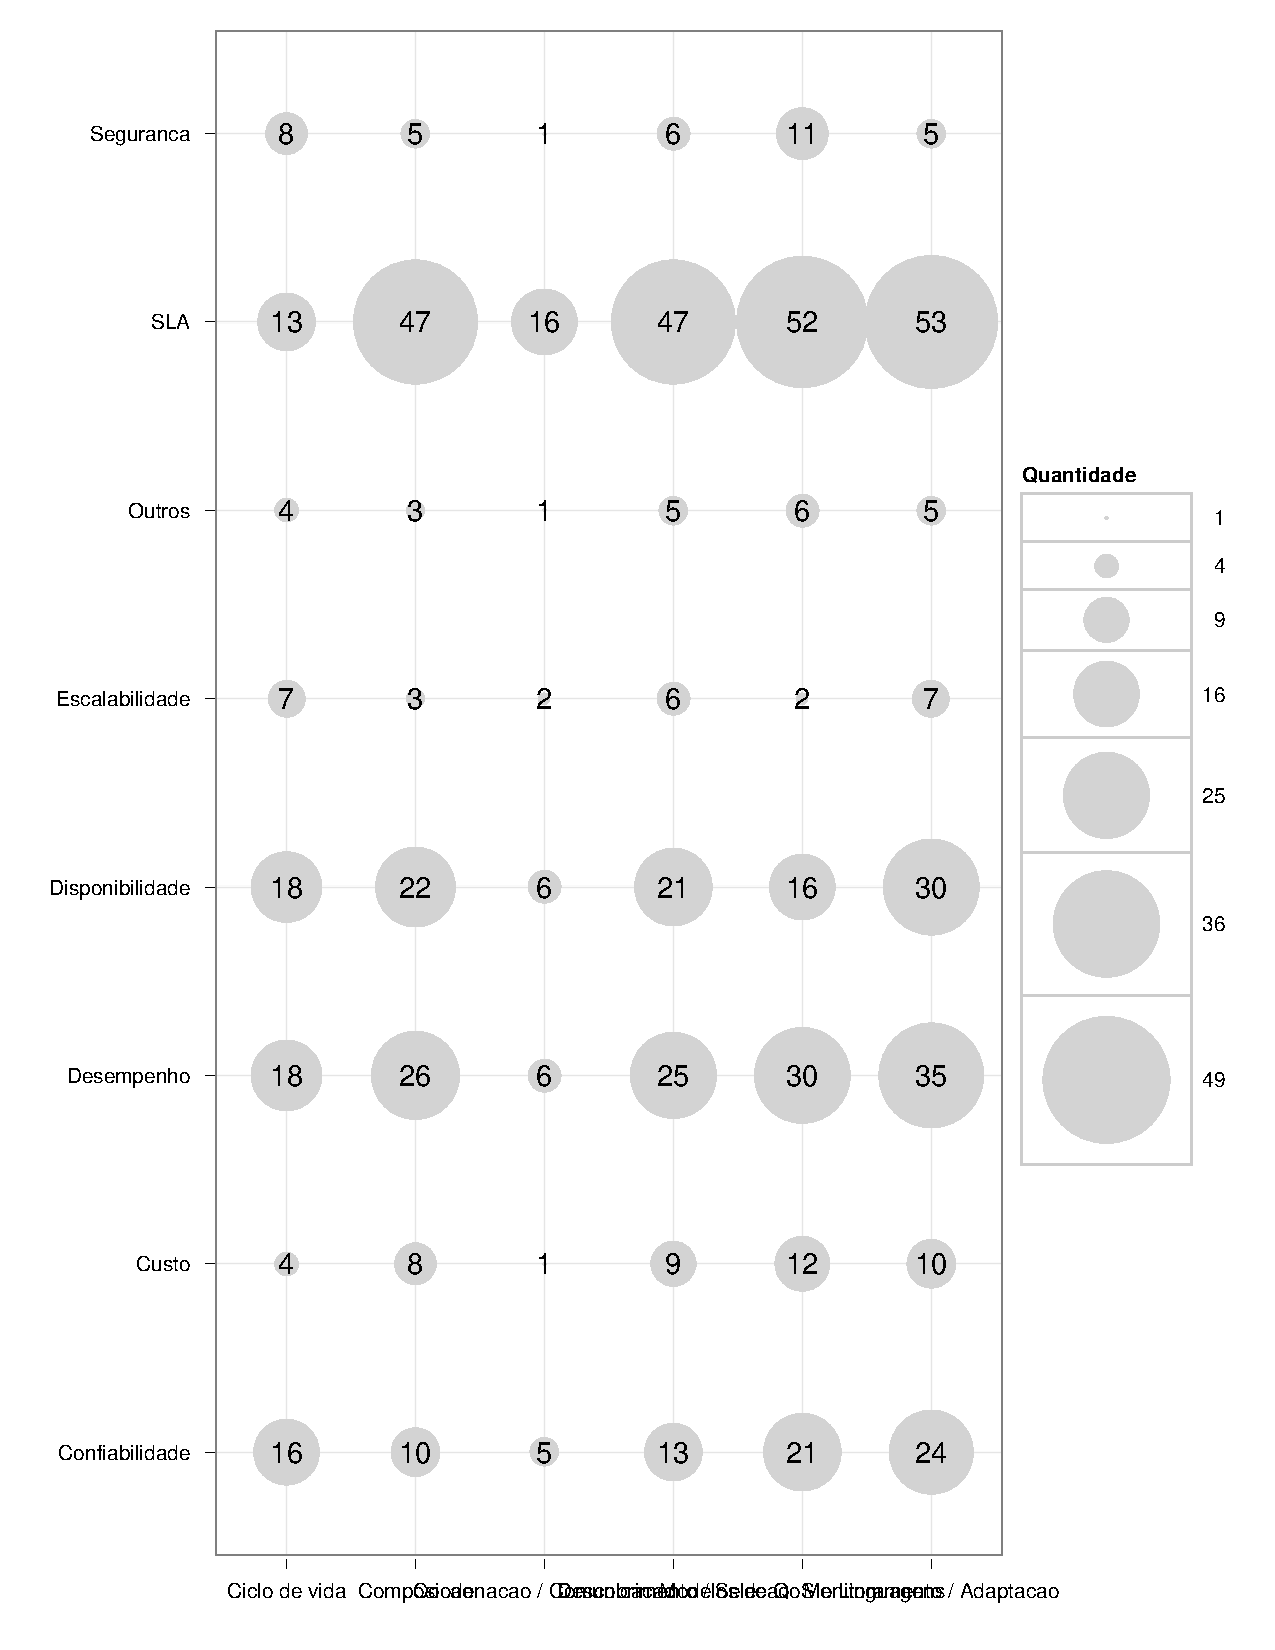
\includegraphics[scale=0.4]{imagens/contribuicaoContexto.pdf}
\caption{\emph{Bubble plot} com a distribui\c{c}\~{a}o ap\'{o}s a realiza\c{c}\~{a}o do primeiro  estudo}
\label{fig:bubbleplot-QoSSOC}
\end{figure}

O resultado desse mapeamento mostra que a maior parte dos trabalhos publicados lida com monitoramento e adapta\c{c}\~{a}o (\MonitoramentoAdaptacao), seguida de modelos de QoS \& linguagens (\ModelosdeQoSeLinguagens), descoberta \& sele\c{c}\~{a}o (\DescobrimentoSelecao),  composi\c{c}\~{a}o (\Composicao), ciclo de vida (\Ciclodevida) e finalmente coordenação com \CoodenacaoComunicacao.

Esses resultados indicam o foco dado a aspectos não funcionais, dinâmicos e que podem sofrer variações devido a concorrência e poss\'{i}veis falhas dos servi\c{c}os em tempo de execu\c{c}\~{a}o. Uma preocupa\c{c}\~{a}o que pode refletir problemas no modelo de terceirização de serviços. Uma outra observa\c{c}\~{a}o: dado que o ambiente SOC possui características próprias e diferenciadas, é natural que novas métricas de QoS tenham sido definidas ou que métricas já utilizadas tenham ganho novos significados, assim como linguagens e especificações que admitam o tratamento e negociação dos requisitos de qualidade. O resultado obtido nesse estudo para o atributo de modelos de QoS e linguagens atesta essa constatação. Nota-se também que a descoberta e seleção de serviços foi bem endereçada nas pesquisas, assim como a composição. No primeiro grupo, é considerado o descobrimento e escolha entre serviços de mesma funcionalidade, porém com diferentes níveis de QoS. O segundo abrange não somente a composição, mas também a escolha da melhor configuração de modo a atender aos níveis globais desejáveis ou necessários de QoS para um conjunto de serviços. Por fim, notou-se um número reduzido de trabalhos que abordam ciclo de vida e menos expressivo ainda com rela\c{c}\~{a}o a coordenação \& comunicação. 

\subsection{Quest\~{a}o de Pesquisa 2}
\emph{Quais atributos de qualidade são frequentemente considerados nos estudos abordados?}

Para responder a essa pergunta, olhamos a distribui\c{c}\~{a}o dos artigos no eixo de QoS, a faceta de contexto. O eixo vertical da Figura~\ref{fig:bubbleplot-QoSSOC} apresenta os resultados dessa distribui\c{c}\~{a}o. Vale ressaltar que, como cada artigo pode tratar de m\'{u}ltiplos atributos de QoS, a soma total do n\'{u}mero de artigos mapeados em cada um dos atributos n\~{a}o totalizar\'{a} o n\'{u}mero de artigos inclu\'{i}dos no mapeamento. Por exemplo, o artigo~\cite{DBLP:journals/tse/CalinescuGKMT11} lida com os atributos de disponbilidade, desempenho e confiabilidade. 

O mapa mostra que SLA (90\% dos artigos) \'{e} o que predomina, seguido de desempenho (59.2\% dos artigos), disponibilidade (49.6\% dos artigos) e confiabilidade (38\% dos artigos). Os atributos menos observados s\~{a}o custo (19.6\% dos artigos), seguran\c{c}a (16.4\% dos artigos) e escalabilidade (13.2\% dos artigos). Os atributos que n\~{a}o se enquadraram especificamente em nenhum desses foram classificados em outros (9.2\% dos artigos) como aqueles que envolvem outros atributos de qualidade como, por exemplo, \cite{6036406} que define um crit\'{e}rio de sele\c{c}\~{a}o de servi\c{c}o conforme sua reputa\c{c}\~{a}o. 

A partir desses resultados, pode-se notar que, no contexto de SOC, os termos mais relacionados a QoS s\~{a}o SLA, desempenho, disponibilidade e confiabilidade, com bastante \^{e}nfase em SLA. No entanto, observamos muitas vezes que os trabalhos mencionavam QoS sem explicitar qual atributo em particular estava em quest\~{a}o. Nesses casos, com base nas m\'{e}tricas utilizadas, classificamos como SLA por ser a op\c{c}\~{a}o mais pr\'{o}xima naquele contexto. Dessa forma, considerando essa classifica\c{c}\~{a}o do SLA como poss\'{i}vel lacuna de clareza nos trabalhos avaliados, os dados gerais nos induzem a concluir que desempenho, disponibilidade e confiabilidade s\~{a}o prioridade como atributos de QoS em SOC. No entanto, o mesmo n\~{a}o pode ser conclu\'{i}do para seguran\c{c}a, escalabilidade e custo. 
\subsection{Quest\~{a}o de Pesquisa 3}
\emph{Quais atributos de qualidade são frequentemente considerados nos estudos abordados?}

Para responder a essa pergunta, olhamos a distribui\c{c}\~{a}o dos artigos no eixo de QoS, a faceta de contexto. A Figura~\ref{Fig:bubbleplot} apresenta o diagrama ilustrando essa distribui\c{c}\~{a}o. Vale ressaltar que, como cada artigo pode tratar de m\'{u}ltiplos atributos de QoS, a soma total do n\'{u}mero de artigos mapeados em cada um dos atributos n\~{a}o totalizar\'{a} o n\'{u}mero total de artigos inclu\'{i}dos no mapeamento. Por exemplo, o artigo~\cite{DBLP:journals/tse/CalinescuGKMT11} lida com os atributos de disponbilidade, desempenho e confiabilidade. 

O mapa mostra que SLA (90\% dos artigos) \'{e} o que predomina, seguido de desempenho (59.2\% dos artigos), disponibilidade (49.6\% dos artigos) e confiabilidade (38\% dos artigos). Os atributos menos observados s\~{a}o custo (19.6\% dos artigos), seguran\c{c}a (16.4\% dos artigos) e escalabilidade (13.2\% dos artigos). Os atributos que n\~{a}o se enquadraram especificamente em nenhum desses foram classificados em outros (9.2\% dos artigos) como aqueles que envolvem outros atributos de qualidade como, por exemplo, \cite{6036406} que define um crit\'{e}rios de sele\c{c}\~{a}o de servi\c{c}o conforme sua reputa\c{c}\~{a}o. 

\subsection{Questão de Pesquisa 4}\label{sub:QP4}

\textbf{Qual o foco da contribuição de pesquisa realizada em SOC e relacionada com qualidade de serviço? }
\\[0.01in]

Com o intuito de responder a esta questão, foi feita uma avalia\c c\~{a}o da distribui\c c\~{a}o dos 
artigos em rela\c c\~{a}o ao tipo de pesquisa (conforme discutido na Se\c c\~{a}o~\ref{sec:review_method}). 
O \emph{bubble plot} na Figura~\ref{fig:bubbleplot-QoSRes}  apresenta tal distibui\c c\~{a}o, novamente sendo importante ressaltar que o n\'{u}mero total de artigos nos gr\'{a}ficos \'{e} superior ao n\'{u}mero total de artigos analisados--- uma vez que alguns artigos apresentam contribui\c c\~{o}es tanto em termos de uma nova solu\c c\~{a}o proposta quanto em termos de avalia\c c\~{a}o e/ou valida\c c\~{a}o. Por exemplo, Huang et al. prop\~{o}e um modelo estoc\'{a}stico para representar e raciocinar sobre dependabilidade em um ambiente de SOC, ao mesmo tempo que valida formalmente tal proposta por meio de provas de teoremas~\cite{huang:scc2011}.

\begin{figure*}[htb]
\centering
\includegraphics[scale=0.55]{imagens/pesquisaContexto3.pdf}
\caption{\emph{Bubble plot} com a distribui\c{c}\~{a}o envolvendo tipos de pesquisa e contexto(QoS)}
\label{fig:bubbleplot-QoSRes}
\end{figure*}

Esta investiga\c c\~{a}o revelou que 155 artigos ou 42.5\% do total apresentam, al\'{e}m de uma nova solu\c c\~{a}o relacionada \`{a} qualidade de servi\c cos em SOC, uma validação da proposta por meio de experimentos e simulações empíricas (e.g.  ~\cite{jeong:fqs2009,ardagna:jss2010,huang:scc2011,binshtok:icsoc2009}). Por outro lado, 163 artigos ou 44.8\% s\~{a}o propostas de solu\c c\~{o}es que não apresentam validações empíricas, isto é, carecem de experimentos que demonstrem a viabilidade e benefícios da(s) técnica(s) propostas. Entre esses artigos podemos citar \cite{filieri:faa2012,nascimento:splc2011,balfagih:icime2011,Clark:2009}. Finalmente, 33 artigos (9\%) foram classificados como avaliação, sendo que 10 apresentam, al\'{e}m de uma nova solu\c c\~{a}o relacionada \`{a} qualidade de servi\c cos em SOC, uma avaliação de técnicas correlatas em casos de uso reais, avaliando as limitações e benefícios das soluções existentes, e 23 artigos (6.3\%) avaliam em casos de uso reais propostas existentes 
identificando seus benefícios e limitações.

Esses n\'{u}meros revelam que a \'{a}rea de pesquisa de qualidade de servi\c co em SOC ainda est\'{a} em uma fase de amadurecimento naquilo que se refere ao uso e adoção em casos de uso reais das propostas, dada o baixo percentual dos artigos classificados como avaliação (9\%), o que indica a necessidade de mais pesquisas capazes de comparar diferentes técnicas já existentes. Também observou-se que um percentual significativo das contribui\c c\~{o}es simplesmente apresentam novas abordagens ou fazem compara\c c\~{o}es envolvendo a pr\'{o}pria t\'{e}cnica proposta (44.8\%).%--- o que refuta nossa hipótese inicial de que pesquisas relativas a QoS em SOC estejam próximas a um patamar de amadurecimento, conforme o ciclo de maturação de Redwine et al. \cite{redwine:icse1985}.

\subsection{Discuss\~{a}o Sobre os Resultados}

Com base nos resultados evidenciados por esse MS, \'{e} poss\'{i}vel
confirmar v\'{a}rios aspectos relevantes. O resultado desse mapeamento
mostra que a maior parte dos trabalhos publicados lida com
monitoramento e adapta\c{c}\~{a}o (34.94\%), seguida de modelos de QoS
\& linguagens (33.73\%), descoberta \& sele\c{c}\~{a}o (28.11\%),
composi\c{c}\~{a}o (27.31\%). Esses resultados indicam o foco dado a
aspectos n\~{a}o funcionais, din\^{a}micos e que podem sofrer
varia\c{c}\~{o}es devido a concorrência e possíveis falhas dos
servi\c{c}os em tempo de execu\c{c}\~{a}o. Mas tamb\'{e}m indicam o
foco em propostas que visam a representa\c{c}\~{a}o e a escolha da
melhor configura\c{c}\~{a}o de modo a atender aos níveis globais
desej\'{a}veis ou necess\'{a}rios de QoS para um conjunto de
servi\c{c}os. 
No contexto de SOC, os dados gerais nos induzem a
concluir que desempenho, disponibilidade e confiabilidade s\~{a}o
prioridade como atributos de QoS em SOC. Seguran\c{c}a,
escalabilidade e custo, no entanto, tiveram menor evid\^{e}ncia no trabalhos analisados em nosso estudo. 
Um futuro estudo com base em cada um desses atributos separadamente pode servir de base para se ter um panorama
mais espec\'{i}fico em cada uma dessas \'{a}reas. Mas entendemos que, devido \`{a} abrang\^{e}ncia de cada um desses t\'{o}picos,
tornar-se-ia invi\'{a}vel tratar dessa quest\~{a}o em nosso estudo. 

Quanto aos grupos que mais contribu\'{i}ram para o contexto de
mapeamento est\~{a}o 3 principais grupos: (1) o S-Cube (com foco em
monitoramento \& adapta\c{c}\~{a}o, assim como composi\c{c}\~{a}o
din\^{a}mica), (2) Menasc\'{e} et al. (com foco em descobrimento \&
sele\c{c}\~{a}o, assim como monitoramento \& adapta\c{c}\~{a}o) e (3)
Lin et al (composi\c{c}\~{a}o din\^{a}mica e
adapta\c{c}\~{a}o). Percebemos tamb\'{e}m que suas
contribui\c{c}\~{o}es se encaixam na \'{a}reas de SOC que mais de
destacaram em nosso estudo. 
Finalmente, em rela\c c\~{a}o ao tipo de pesquisa em
qualidade de servi\c{c}o em SOC, consideramos que a mesma ainda
est\'{a} em uma fase de amadurecimento, 
onde um percentual significativo das contribui\c{c}\~{o}es
simplesmente apresentam 
novas abordagens ou fazem compara\c{c}\~{o}es envolvendo a 
própria t\'{e}cnica proposta. Na pr\'{o}xima se\c c\~{a}o apresentamos
algumas amea\c cas \`{a} validade do nosso estudo, bem como as
estra\'{e}gias que seguimos para que as mesmas
fossem contornadas.

